Una vez definido el algoritmo, se va a explicar la implementación que se ha llevado a cabo teniendo en cuenta las ventajas y limitaciones de la arquitectura. En este caso, orientar el diseño a una FPGA va a condicionar en gran medida la toma de decisiones en este aspecto. 

\begin{figure}[!ht]
\begin{center}
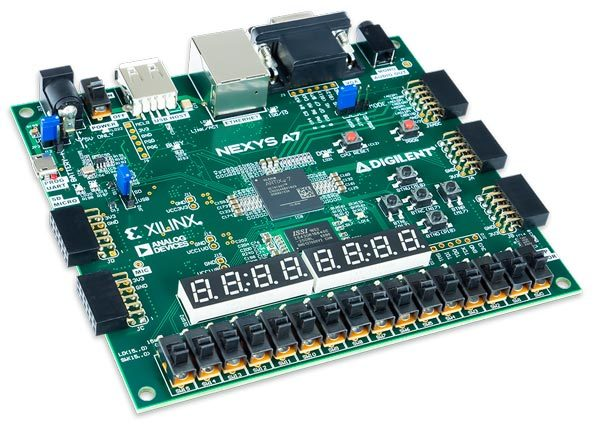
\includegraphics[width=10cm]{img/nexysa7.jpg}
\caption{\label{fig:nexys}Placa Nexys A7}
\end{center}
\end{figure}

Para el montaje de prototipo, se va a utilizar la placa proporcionada por el departamento: Nexys A7 de Digilent, mostrada en la figura \ref{fig:nexys}. Esta placa monta una FPGA de la familia Artix-7 modelo \emph{XC7A100T-1CSG324C} junto con múltiples añadidos para conectividad, entrada y salida de datos, sensor de temperatura y acelerómetro. Además incluye varios diodos LED, que junto a los botones y conmutadores, permiten un cómodo manejo del conjunto de la placa. El conjunto de las prestaciones será más que suficiente para probar más adelante el funcionamiento del prototipo.

De especial trascendencia para la puesta en marcha del conjunto, serán las bahías de pines que se ubican en ambos laterales de la Nexys, puesto que permiten conectar y leer los voltajes de entrada y salida de las señales que se utilizarán. La documentación proporcionada por Digilent \cite{Nexys} ha resultado muchas veces insuficiente, pero fundamental a la hora de poner en marcha el prototipo.

\section{Gestión entrada-salida}
Siguiendo el flujo de datos desde la etapa analógica, el primer paso consiste en introducir los mismos en la FPGA. Para ello, es imprescindible convertir el voltaje analógico en la señal digital mediante el uso de un \emph{Conversor Analógico a Digital}, en lo sucesivo ADC. La Nexys A7 no incorpora ninguno integrado por lo que habrá que conectarlo externamente. Análogamente, será necesario también un \emph{Conversor Digital a Analógico}, o DAC, para reconvertir la salida de audio procesado en tensión analógica . Por ello, se decide buscar ambos conversores conjuntamente, para simplificar su puesta en marcha.

Existen infinidad de conversores de este tipo en el mercado, todos ellos ideados para operar en diferentes condiciones de trabajo, en diferentes formatos y a un precio muy asequible. En el caso de las señales de audio, la mayor especificación que deben de cumplir es el compromiso de la tasa de muestreo $t_{s}$ (o más frecuentemente su inversa, la \emph{frecuencia de muestreo} $F_{s}$) para no corromper la señal entrante y preservar su calidad \cite{samplerate}. Típicamente se utilizan algunos valores ya estandarizados por las grandes empresas a lo largo del siglo XX:

\begin{itemize}
\item \textbf{$F_{s} = 8~kHz$:} Utilizada especialmente para telefonía, aunque no tan común en componentes de audio musical.
\item \textbf{$F_{s} = 22050~Hz$:} Frecuencia de muestreo típica de radio que permite reproducir señales con componentes máximas de hasta 10kHz.
\item \textbf{$F_{s} = 32~kHz$:} Se utiliza escasamente en algunos formatos de vídeo digital, como el miniDV.
\item \textbf{$F_{s} = 44,1~kHz$:} La más extendida en formatos como MP3, MPEG y CD por razones tanto históricas como prácticas. Como un oído joven es capaz de percibir tonos de hasta 20kHz, se estableció esta cifra tras aplicar el criterio de Nyquist junto con un pequeño margen.
\item \textbf{$F_{s} = 48~kHz$:} También muy utilizada en televisión digital, DVD y audio profesional.
\item \textbf{$F_{s} = 96~o~192,4~kHz$:} Pensada especialmente para audio de alta definición en formatos como HD-DVD y Blue-Ray Disc
\end{itemize}

Tras analizar las posibilidades, resulta evidente que para una aplicación musical conviene establecer la frecuencia de muestro en 44,1 o 48 kHz de forma que conserve cierta similitud con los equipos comerciales y profesionales del mercado \cite{cdsamp}.

Así, aprovechando su reciente adquisición por parte del departamento, se va utilizar un componente que integre tanto ADC como DAC y que permita trabajar a estas velocidades: el \emph{Pmod i2-s2}, también de Digilent.

\subsection{Pmod i2-s2}
Este componente contiene todo lo necesario para este proyecto: junto a los ADC y DAC incorpora dos puertos para mini-jack estéreo hembra\footnote{Lo más extendido para audio, puesto que son los conectores que llevan móviles, auriculares. ordenadores, etc...} y una serie de pines dispuestos de tal forma que la conexión con la placa es inmediata. Se pueden observar estas características en la imagen \ref{fig:pmod}.

\begin{figure}[!ht]
\begin{center}
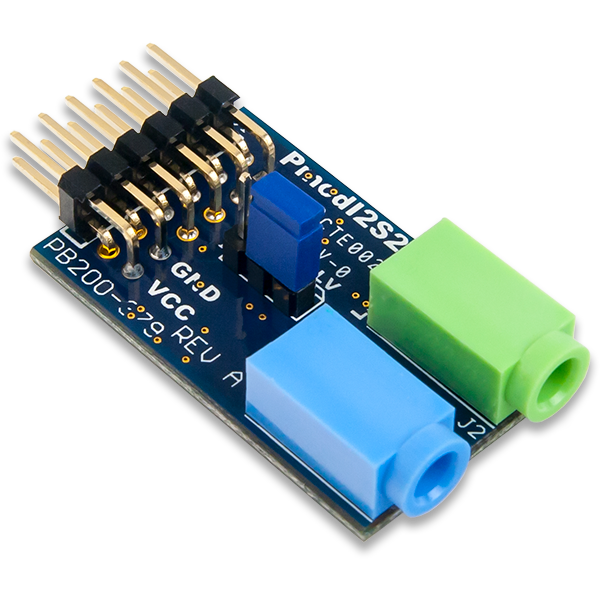
\includegraphics[width=5cm]{img/pmod.png}
\caption{\label{fig:pmod}Detalle del Pmod i2-s2}
\end{center}
\end{figure}

Como tanto la placa como el \emph{plug-in} son productos de Digilent, no hay ningún problema a la hora de interconectarlos, basta con insertarlo en una de las bahías de pines que tiene la FPGA. Además, las conexiones de alimentación: Vcc y GND, se encuentran hechas de serie en la Nexys, por lo que no es necesario añadirlas en el fichero de conexiones o \emph{constraints}.

Tanto el modelo de ADC, \emph{Cirrus CS5345} \cite{adcdata}, como el de DAC, \emph{Cirrus CS4344} \cite{dacdata} realizan las conversiones con hasta 24 bit por muestra e incorporan un filtro paso bajo anti-aliasing que por tanto, no hará falta implementar. Además tienen 98 dB de rango dinámico y baja distorsión armónica, haciéndolos ideales para las aplicaciones de audio, aún más cuando están conectados a  las entradas de \emph{mini-jack}.

Aunque los conversores soportan hasta 24 bit, el tamaño de cada palabra de datos será de 16 bit, debido a que es la longitud que utiliza el formato CD y aumentar este tamaño resulta costoso en recursos. La otra diferencia con respecto a este formato será que el procesado será \emph{mono} en lugar de \emph{estéreo}. Evidentemente, la existencia de dos canales dobla el número de operaciones y la complejidad del algoritmo al tener que duplicar el flujo de datos en todos los puntos del diseño. Por ello, no se suelen utilizar conexiones ni procesados estéreo en aplicaciones de audio en tiempo real, especialmente en instrumentos monofónicos\footnote{Instrumentos que solo pueden producir una nota al mismo tiempo}. Normalmente, estos instrumentos tienen un lugar fijo en la panorámica de la producción, siendo esta la razón por la cual el procesado estéreo no se suele emplear. En la práctica, se muestrearán los datos del canal izquierdo, que por convenio es el principal cuando se opera solo con un canal, y tras el procesado, se escribirá el resultado en ambos canales.

\subsection{Consideraciones de la implementación del Pmod}
Generalmente, se ha recurrido a la documentación del fabricante, \emph{Cirrus Logic} en el caso de los conversores o \emph{Artix} en el caso de la FPGA en lugar de 1 la proporcionado por Digilent, que resulta ser en muchos casos poco concisa e incompleta.

Tras insertar el Pmod en la bahía de pines, se debe modificar el archivo de conexiones~\emph{.xdc}.Es recomendable buscar este archivo en la página de la Nexys A7\footnote{En algunos ejemplos de Digilent en GitHub el numerado de los pines es incorrecto, por lo que hay que actuar con cautela.}. Hay que recordar que el lenguaje de este tipo de archivos es \emph{case sensitive}, es decir, que a diferencia del VHDL distingue entre minúsculas y mayúsculas. En este tipo de ficheros tampoco puede haber dos señales con el mismo nombre, si es necesario duplicar una señal (que lo será en varios relojes) debe hacerse desde el código principal VHDL para posteriormente nombrarlo diferente de cara a las conexiones. 

\begin{figure}[!ht]
\begin{center}
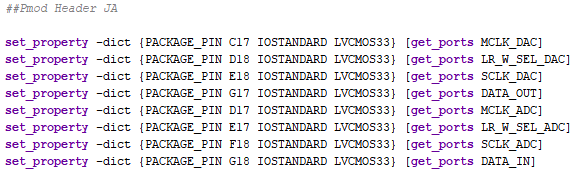
\includegraphics[width=12cm]{img/xdc.png}
\caption{\label{fig:xdc}Conexiones del Pmod con la FPGA en el fichero .xdc}
\end{center}
\end{figure}

La comunicación entre ambos módulos sigue un protocolo $I^{2}S$ \cite{i2s} el cual está extendido en este tipo de componentes. Este protocolo separa la señal de datos del resto de señales de reloj, de forma que se garantiza su funcionamiento síncrono. Así, la FPGA actúa como dispositivo maestro generando estas señales y tanto el ADC como el DAC lo hacen como esclavos. Los relojes utilizados serán los siguientes:

\begin{itemize}
\item \textbf{MCLK:} Es el reloj maestro del sistema a partir del cual se van a generar el resto. De este reloj depende el funcionamiento de la lógica interna del Pmod.
\item \textbf{SCLK:} Corresponde al reloj de bit, es decir, cada periodo equivale a la duración de un bit al leer o escribir. Este reloj está en contrafase con el resto.
\item \textbf{LRCK:} Conmuta con la variación canal, es decir, cuando LRCK = 1 se realizan operaciones sobre el canal derecho y cuando LRCK = 0 sobre el izquierdo, de forma que su lectura es alterna. Como se lee una palabra en cada semperiodo del reloj, su frecuencia será siempre el doble de la frecuencia de muestreo. Para evitar confusiones en el proyecto de Vivado se ha cambiado su nombre a LR\_W\_SEL.
\end{itemize}

Es fundamental entender que las relaciones entre estos tres relojes aseguran tanto la correcta interpretación de los datos y su reconstrucción como la comunicación con el módulo maestro, la FPGA. Para este proyecto se ha fijado una frecuencia de \textbf{50~MHz} para MCLK, ya que de esta forma es más sencilla su relación con el reloj de sistema de 100~MHz. Para el resto de relojes, hay que consultar la tabla de equivalencias proporcionada por el fabricante, imagen \ref{fig:flujoreloj}.

\begin{figure}[!th]
\begin{center}
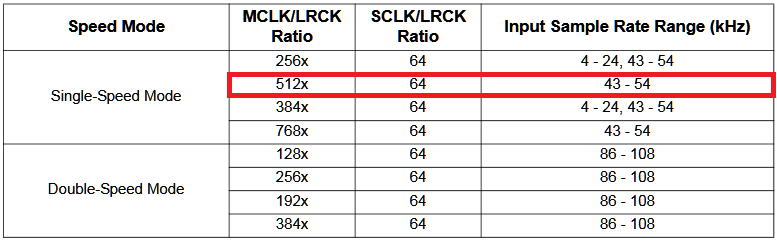
\includegraphics[width=15cm]{img/ratiosreloj.png}
\caption{\label{fig:flujoreloj}Tabla de las relaciones entre los relojes}
\end{center}
\end{figure}

\begin{figure}[!th]
\begin{center}
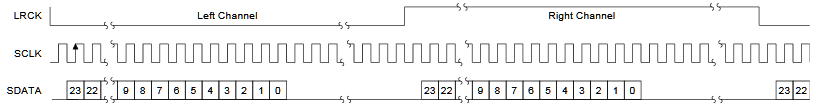
\includegraphics[width=14cm]{img/i2sov.png}
\caption{\label{fig:i2sov}Funcionamiento de los relojes de control con flujo de datos}
\end{center}
\end{figure}

Como la frecuencia de MCLK es fija dada por el sistema, para obtener la frecuencia de muestreo deseada en torno a los 44,1~kHz, hay que aplicar el factor 512. De esta forma si $F_{MCLK}~=~50~MHz$ entonces $F_{LRCK}~=~F_{MCLK}/512 = 97.656,25~Hz$ pero compartida entre los dos canales. Por tanto $F_{s}$ de un canal resulta $F_{s} = 97.656,25/2 = 48.828,125 Hz \approx 48,8 kHz$. Finalmente, como el factor $F_{SCLK}/F_{LRCK}=64$ obtenemos $F_{SCLK}~=~3,135~MHz$. Como se puede ver, la frecuencia de muestreo obtenida es mayor que la buscada y necesaria, pero se asemeja al estándar de alta calidad, por lo que tampoco se decide modificarla. Para generar estas frecuencias se barajó la opción de utilizar el \emph{clocking wizard}, un módulo IP de Vivado que garantiza la correcta generación de varias señales de reloj salientes a partir de una entrante. Sin embargo, este no admite valores inferiores a las decenas de megahercios. Por ello se ha tenido que implementar un contador que permitiera dividir la frecuencia en múltiplos de 2 usando los bit de esa señal. El pseudocódigo se muestra en la figura \ref{fig:controlsig}.

\begin{figure}[!h]
\begin{center}
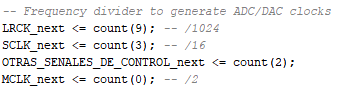
\includegraphics[width=7cm]{img/controlsig.png}
\caption{\label{fig:controlsig}Esquema de la generación de los relojes}
\end{center}
\end{figure}

La adquisición de los datos se completa usando un registro de desplazamiento propuesto por P.Chu \cite{vhdlchu}. El primer bit, que será el más significativo o MSB, se lee un ciclo después de que conmute LRCK, como se muestra en la figura \ref{fig:i2sov}. \textbf{El resultado son palabras de 16 bit en complemento a 2 normalizadas en el intervalo (-1,1).}

\section{Controlador de datos}
Una vez establecido el flujo de entrada/salida, se puede comenzar el desarrollo del procesado. Primeramente es necesario adecuar las palabras recibidas para su correcta interpretación y transformarlas al dominio de la frecuencia. Una vez realizadas todas las operaciones sobre ellas, se realiza la transformada inversa y su reconstrucción. La figura~\ref{fig:dbloques} muestra estas etapas junto con el tamaño de palabra asociado en cada punto. Hay que notar que debido a las diferentes frecuencias de funcionamiento los módulos funcionan a velocidades distintas, por lo que la escala temporal está distorsionada en esa figura. Esa es la razón por la cual el número de flechas de entrada y salida no coincide entre todos los bloques.

\begin{figure}[!ht]
\begin{center}
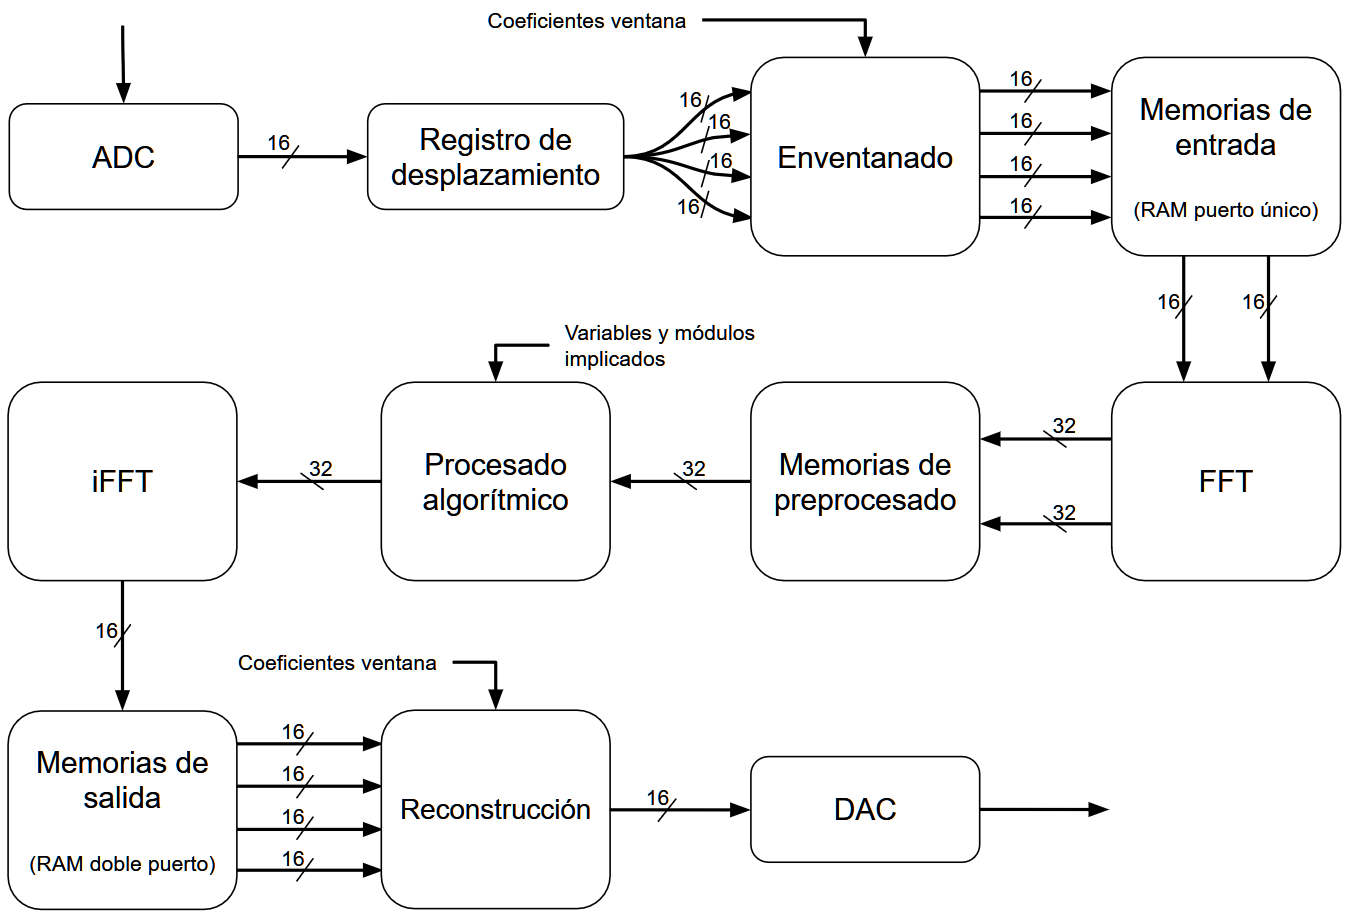
\includegraphics[width=15cm]{img/diagramabloques.png}
\caption{\label{fig:dbloques}Diagrama de bloques del procesado en la FPGA}
\end{center}
\end{figure}

El encargado de gestionar el flujo de datos de entrada/salida es el llamado \emph{master\_controller}. Este se encarga de generar las señales necesarias para el correcto funcionamiento de Pmod y de instanciar el resto de componentes que se utilizarán, a excepción de los displays. Para garantizar el flujo de datos apropiado, se modela mediante una máquina de estados cuyo esquema corresponde a la figura \ref{fig:estados}. La lógica del cambio de estados se ubica en un fichero aparte llamado \emph{fsm\_control}. Los cambios de estado los produce la variable \emph{frame\_number}, la cual se encarga de llevar la cuenta de los ciclos de reloj de bit (SCLK) que se producen en cada flanco del reloj de canal (LRCK) hasta un total de 32. En principio se cumple este diagrama solo para el canal izquierdo, es decir, cuando LR\_W\_SEL = 0, aunque veremos que esto podrá variar. A continuación se describen cada uno de los estados: 

\begin{itemize}
\item \textbf{IDLE:} Es el estado fundamental aunque no de reposo, ya que se activa el registro de desplazamiento para leer el dato proveniente del ADC quedando almacenado en un búfer.
\item \textbf{WRITE\_INPUT:} Lee el búfer donde está escrito el dato de entrada proveniente del ADC, le aplica el factor de enventanado que le corresponda y lo almacena en memoria.
\item \textbf{LOAD\_FREQ:} Traslada el dato de la memoria donde estaba almacenado al módulo que realiza la FFT. Como la velocidad de procesado es mucho más rápida que la frecuencia de muestreo, se evitarán las colisiones.
\item \textbf{UNLOAD\_FREQ:} Devuelve el dato procesado proveniente del módulo que realiza la iFFT y lo almacena en una memoria de salida.
\item \textbf{READ\_OUTPUT:} Lee los cuatro datos de las memorias de salida y los almacena en otros registros temporales.
\item \textbf{READ\_SUM:} Aplica la ventana de salida a las cuatro muestras ubicadas en los registros y las suma entre sí para obtener el dato que se va a escribir en el siguiente ciclo, el cuál se guarda nuevamente en un registro.
\end{itemize}

\begin{figure}[!th]
\begin{center}
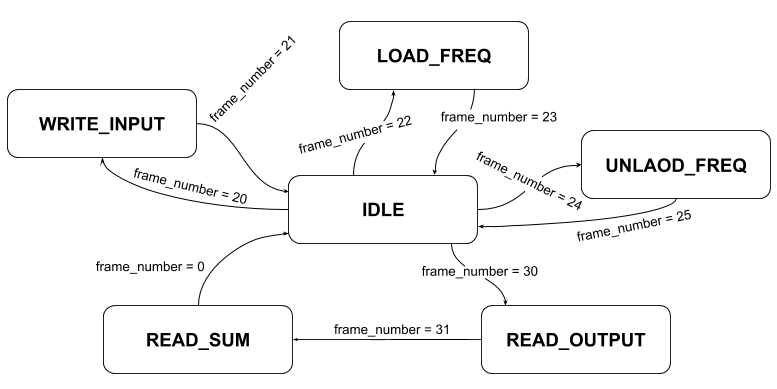
\includegraphics[width=13cm]{img/destados.png}
\caption{\label{fig:estados}Diagrama de estados del controlador de datos}
\end{center}
\end{figure}

Salta a la vista que son necesarios varios bancos de memorias, cada uno ubicado en un punto diferente del flujo de datos. La implementación de cada uno de ellos varía en función de su propósito, como se verá a continuación en \ref{memo}. Sin embargo, conviene primero aclarar cómo se lleva a cabo el proceso de enventanado, ya que condiciona en gran medida el diseño del flujo de datos.

\subsection{Implementación del solapamiento}
Como se ha descrito anteriormente, el factor de solapamiento que se va utilizar es del 75\%. Esto quiere decir que serán necesarias al menos cuatro memorias para poder almacenar toda la información, tal y como se muestra en la figura \ref{fig:solap}. 

\begin{figure}[!b]
\begin{center}
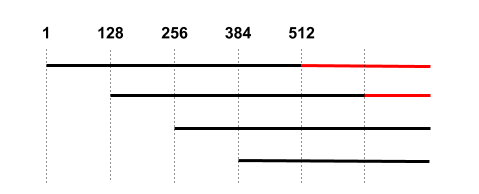
\includegraphics[width=13cm]{img/solap.png}
\caption{\label{fig:solap}Esquema del solapamiento entre las memorias}
\end{center}
\end{figure}

Cada una de las barras horizontales representa una de las cuatro ventanas que se almacenarán en espacios de memoria diferentes. Es importante asegurar que la muestra entrante se multiplica por el coeficiente de enventanado adecuado, que depende exclusivamente de la posición de la muestra respecto a la ventana. De esta forma, la palabra entrante se registra una vez para luego ser multiplicada por la constante de enventanado de cada ventana antes de ser almacenada en su memoria correspondiente.

En el momento de la reconstrucción, es necesario hacer cuatro accesos a memoria que recuperen cada uno de los cuatro datos procesados para multiplicar nuevamente por la constante apropiada y sumarlos todos entre sí. Los valores de las constantes de ambas ventanas garantizan que no haya desbordamiento en esta suma.

Los coeficientes de enventanado que se utilizan durante el procesado se almacenan en dos memorias no volátiles, una para la etapa previa a la FFT y otra para la posterior la iFFT, las cuales se corresponden con las etapas de enventanado y reconstrucción respectivamente. Estas memorias se generan utilizando únicamente lógica combinacional en VHDL para minimizar la latencia de las mismas. Para no introducir todos los valores de forma manual se ha creado un script de Matlab que escribe los ficheros automáticamente, cuyo código se encuentra en el apéndice \ref{ap:script}.

\subsection{Bancos de memorias volátiles\label{memo}}
Todas las memorias volátiles del proyecto están implementadas utilizando los módulos de Vivado \emph{Block Memory Generator}. Estos asistentes permiten crear memorias RAM y ROM e inicializarlas a un valor determinado usando un fichero de texto. Únicamente se van a utilizar dos tipos de RAM generadas de este manera cuyo esquema se muestra  en la figura \ref{fig:rams}.

En el caso de las memorias de entrada, está garantizado que no existan colisiones tanto en el proceso de lectura como en el de escritura, por lo que se puede utilizar el diseño más simple que propone Vivado: las memorias RAM de puerto único \cite{ram}. Este tipo de memorias poseen un puerto \emph{WEA} que conmuta la posición de lectura y escritura. Como hay un estado para escribir y otro para leer, el valor de WEA va a conmutar como una señal de salida de tipo Moore de la máquina de estados asociada y consecuentemente nunca se van a corromper los datos. En general, se utilizarán este tipo de memorias siempre que se pueda debido a su simpleza, aunque se debe asegurar que no se produzcan colisiones.

\begin{figure}[!b]
\begin{center}
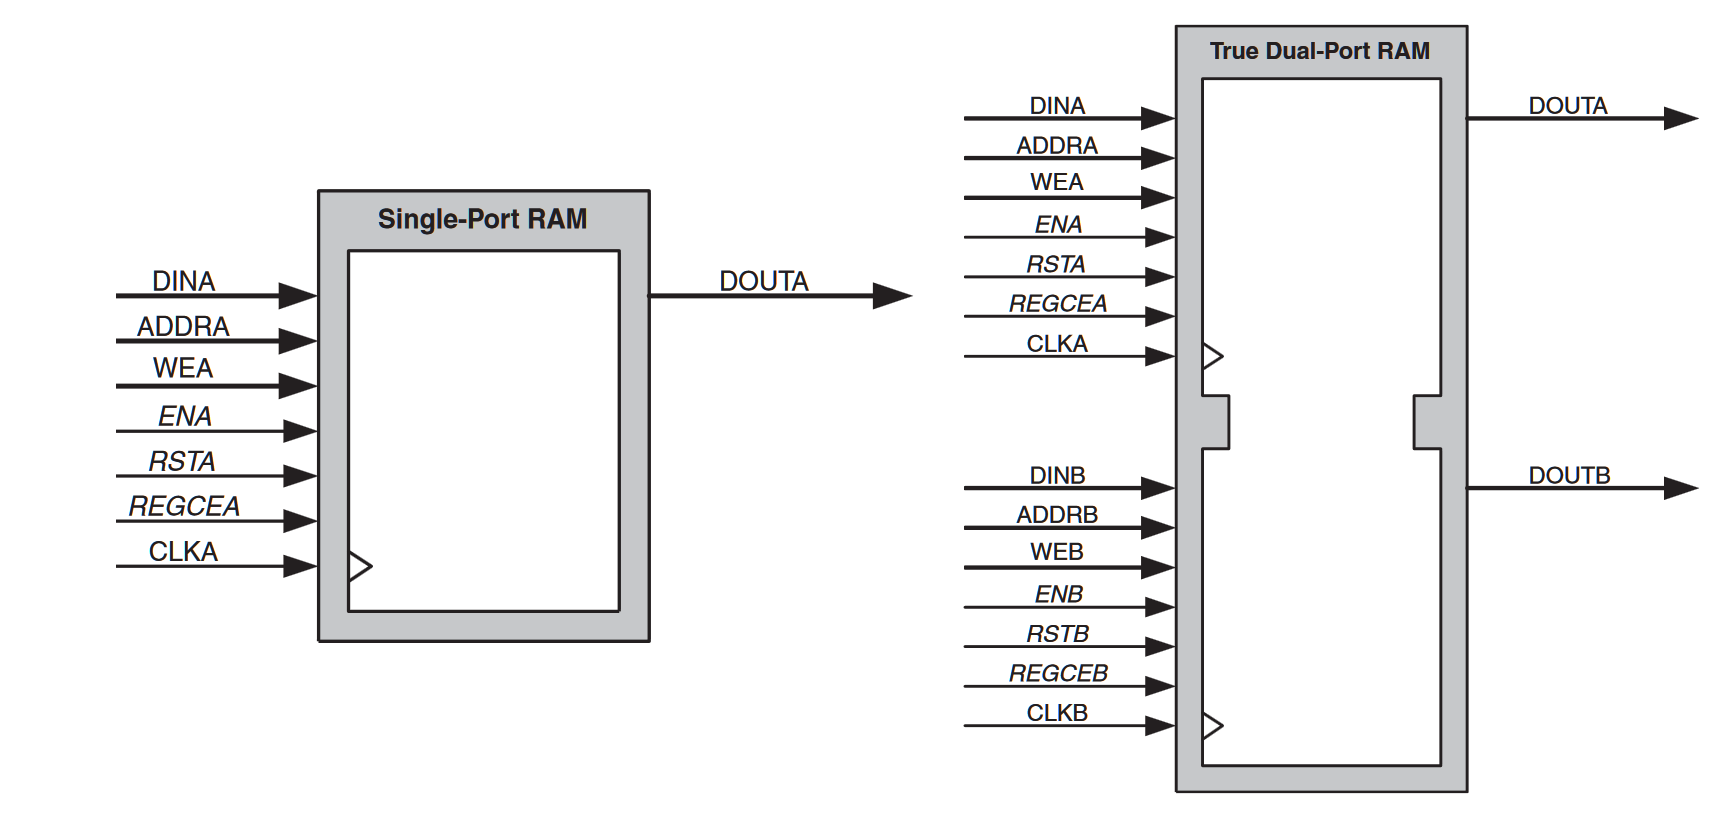
\includegraphics[width=12cm]{img/rams.png}
\caption{\label{fig:rams}Tipos de memorias RAM implementadas}
\end{center}
\end{figure}

Las memorias RAM de puerto doble (derecha en la figura \ref{fig:rams}) funcionan practicamente de la misma manera, salvo que poseen los puertos de entrada y salida duplicados. De esta forma se puede leer y escribir en el mismo instante, siempre que sea en direcciones diferentes. Este tipo de memorias serán adecuadas cuando la lectura y escritura no estén claramente diferenciadas en el tiempo, por ejemplo, en el caso de la salida. Tras el procesado inverso de la iFFT, las muestras deben almacenarse en memoria de forma continua, sin interrupción, lo que podría causar problemas si justo en ese momento fuera necesario leer una muestra para escribirla en el búfer de salida. Esto es la consecuencia de no realizar todas las operaciones bajo el mismo periodo de reloj: mientras que el muestreo se realiza a frecuencia $F_{s}=48,8kHz$, el reloj general del sistema tiene una frecuencia $F_{clk} = 100MHz$. La razón para realizar esta conversión es que si todo el sistema trabajase a la frecuencia de muestreo, el procesado FFT requeriría mucho más tiempo para llevarse a cabo, aumentando en gran medida la latencia. 

Ambos tipos de memorias poseen las mismas características, salvo que dependiendo del lugar que ocupen en la cadena de datos, el tamaño de la palabra y el número de direcciones que poseen varían. Es importante tener en cuenta que estas memorias tienen un \emph{pipeline} interno que provoca un retraso de 2 ciclos en la lectura, ciclos durante los cuales es necesario mantener la señal de \emph{enable} activa. La documentación que proporciona Xillinx y los ficheros auxiliares que se generan al sintetizar estos módulos facilitan el correcto tratamiento y configuración de los bloques de memorias.

\subsection{Core FFT e iFFT\label{ap:FFT}}
Análogamente, se ha utilizado el módulo de Vivado \emph{Fast Fourier Transform v9.0}~\cite{fftdoc} para realizar las transformaciones de Fourier al dominio de la frecuencia. Aunque existe la posibilidad de utilizar más de un canal para llevar a cabo varias operaciones de forma simultánea, he preferido utilizar varios módulos monocanal ya que de esta forma se pueden configurar más fácilmente y simplificar el flujo de datos, a cambio de área en la FPGA. Dado que existen 4 ventanas, parece que serán necesario 4 pares FFT-iFFT, sin embargo, debido a la diferencia de velocidad en el procesado podemos utilizar únicamente 2 de estos pares. Así las ventanas pares compartirán un módulo FFT y las impares el otro. La figura \ref{fig:esq_fft} muestra el esquema temporal que se va a implementar para permitir esta operativa donde el azul representa la carga del módulo par y el amarillo del impar.
 
\begin{figure}[!hb]
\begin{center}
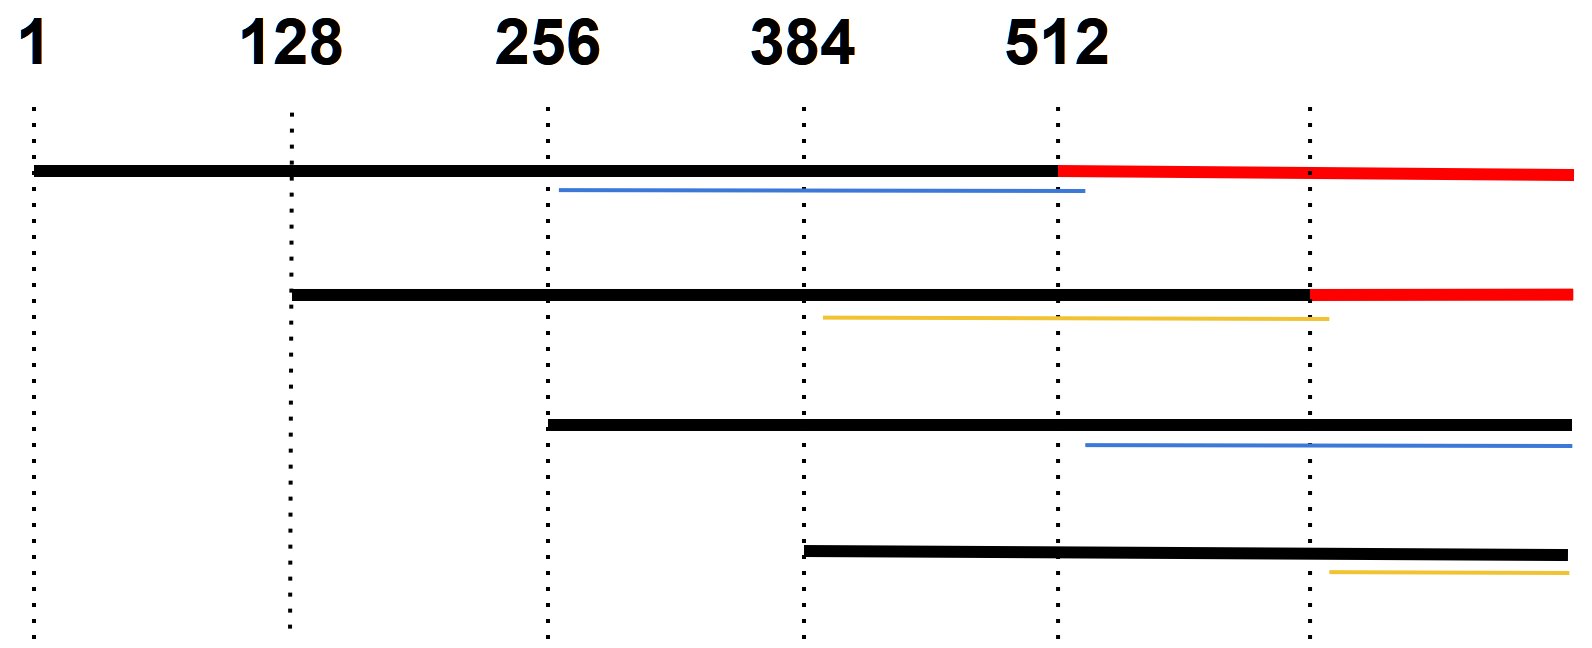
\includegraphics[width=12cm]{img/esqfft.png}
\caption{\label{fig:esq_fft}Esquema temporal de la carga de las FFT}
\end{center}
\end{figure}

En este esquema, la carga de los módulos FFT ocupa exactamente la mitad del tiempo que se emplea para leer los datos de una ventana. Esto se garantiza en la máquina de estados utilizando los ciclos del canal que no está en uso de forma que hay dos ciclos de carga FFT por cada uno de los de llenado de memoria.

La configuración de cada uno de estos módulos se orienta a mejorar lo más posible la latencia, para lo que se establece una longitud de transformada de 512 puntos y una arquitectura con \emph{pipeline} en formato de punto fijo. Se utilizarán 16 bit para parte real y otros 16 para parte imaginaria de forma que al final de cada etapa interna se redondeen los valores, en lugar de truncarlos. Además, para asegurar que no se produzca \emph{overflow} o desbordamiento en ninguna de estas etapas se va a realizar un escalado por un factor 8, aunque el valor de este se puede configurar en tiempo real por medio de una señal destinada a tal fin: \emph{s\_axis\_config\_tdata} (ver figura \ref{fig:mod_fft}). Esta misma señal es la que contiene la información sobre el sentido de la transformada. 
\begin{figure}[!ht]
\begin{center}
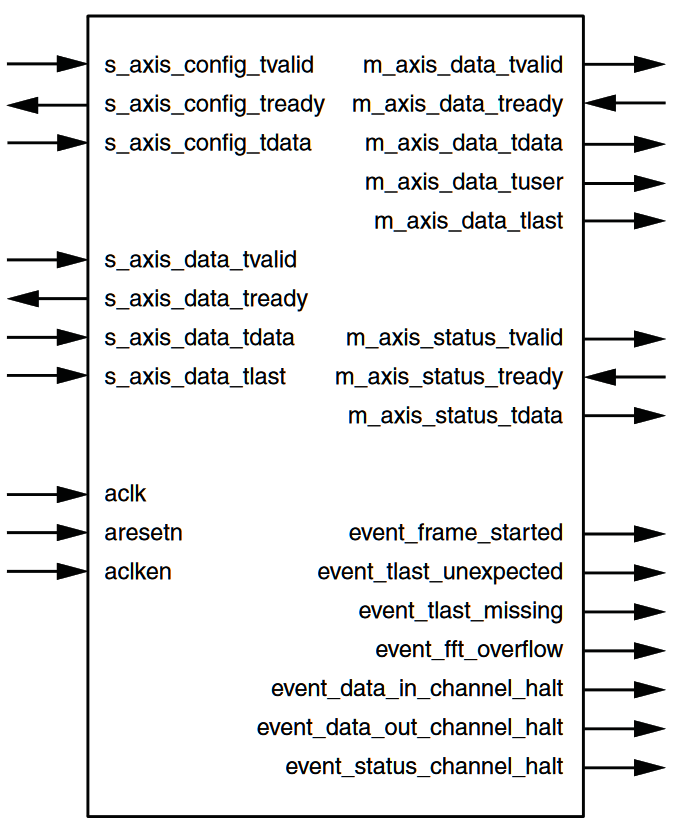
\includegraphics[width=8cm]{img/modulofft.png}
\caption{\label{fig:mod_fft}Diagrama de señales del módulo FFT de Vivado}
\end{center}
\end{figure}
Para intercambiar satisfactoriamente la información de las señales de datos se sigue siempre el mismo protocolo. Cuando el maestro va a proceder a enviar el dato, conmuta la señal \emph{VALID} a 1, si el esclavo está listo para recibir el dato, entonces la señal \emph{READY} se establece a 1. Solo cuando ambas señales \emph{VALID} y \emph{READY} valgan 1, se producirá el intercambio. Este protocolo se aplica a la entrada y salida de datos, a la entrada de configuración y a la salida de \emph{estatus}, la cual no va a ser utilizada debido a la configuración de nuestros módulos.

Las señales de eventos son de gran utilidad especialmente para hacer \emph{debug} del código y ponerlo a punto. En concreto, la señal de comienzo de trama (\emph{event\_frame\_started}) y las de final (\emph{event\_tlast\_unexpected} y \emph{event\_tlast\_missing}) son las que hay que tener en cuenta para comprobar si se ha introducido la trama correctamente. Aún así, pueden inducir a error debido a que el módulo tiene un \emph{pipeline} interno de $n=\log_{2}(l_{FFT})/2$ etapas, redondeando hacia arriba.\footnote{En este caso el \emph{pipeline} tiene $\log_{2}(512)/2 = 4.5 \rightarrow 5$ etapas} Consecuentemente, las señales de los diferentes eventos se observan en la salida con 5 ciclos de retraso respecto al momento en el que se produce dicho evento, lo que es importante a la hora de validarlas.

Cabe destacar que los núcleos FFT poseen memorias internas de entrada y salida que favorecen el intercambio de datos con facilidad. Mediante el correcto uso de la señal \emph{VALID} de la entrada de datos se va a pausar la carga de los mismos de forma que únicamente se vuelquen muestras durante los estados destinados a tal fin. El procesado, en cambio, se lleva a cabo sin tener en cuenta el estado de \emph{master\_controller}. Contrariamente, el resultado de la transformación se va a guardar en memoria inmediatamente después de haberse generado.

Debido a que la operativa sobre la fase no se ha implementado en VHDL, no se ha estudiado con detenimiento cómo resulta más conveniente hacer la carga de datos al módulo iFFT, pero como el tiempo de procesado va a ser elevado\footnote{Conviene recordar que para procesar una muestra es necesario conocer la trama siguiente} lo más sencillo sería ir introduciendo los datos de salido según se fueran generando. Así los núcleos FFT e iFFT funcionarían de la misma manera.

Por último, la salida de las muestras procesadas por la iFFT en el dominio del tiempo, se almacenan en la memoria de doble puerto mencionada con anterioridad para que este disponible en el momento en que la escritura deba llevarse a cabo.

\section{Controlador global}
El controlador global del sistema recibe el nombre de \emph{fsm\_global} y también utiliza una máquina de estados para gestionar el estado del dispositivo. Para esta versión inicial del prototipo, la máquina implementada es muy sencilla ya que únicamente dispone de una función de \emph{pause}. De cara al futuro, el resto de mejoras del pedal en cuanto a manejo y control deberían implementarse en esta máquina de estados. Un ejemplo puede ser la incorporación de un control de volumen o de panorámica estéreo. Si se deseara habilitar más opciones de control como un botón o vincular alguna información a los LED, también habría que realizarlo aquí.

Este fichero es el \emph{TOP} de la arquitectura, por lo que las señales entrantes y salientes que precise, deberán provenir o dirigirse únicamente a la FPGA, utilizando para ello el fichero de conexiones~\emph{.xdc}. Los archivos de \emph{testbench} que se empleen con el objetivo de probar el conjunto del sistema también deben referirse a este archivo, especialmente para la simulación post-síntesis o post-implementación. 

\begin{figure}[!ht]
\begin{center}
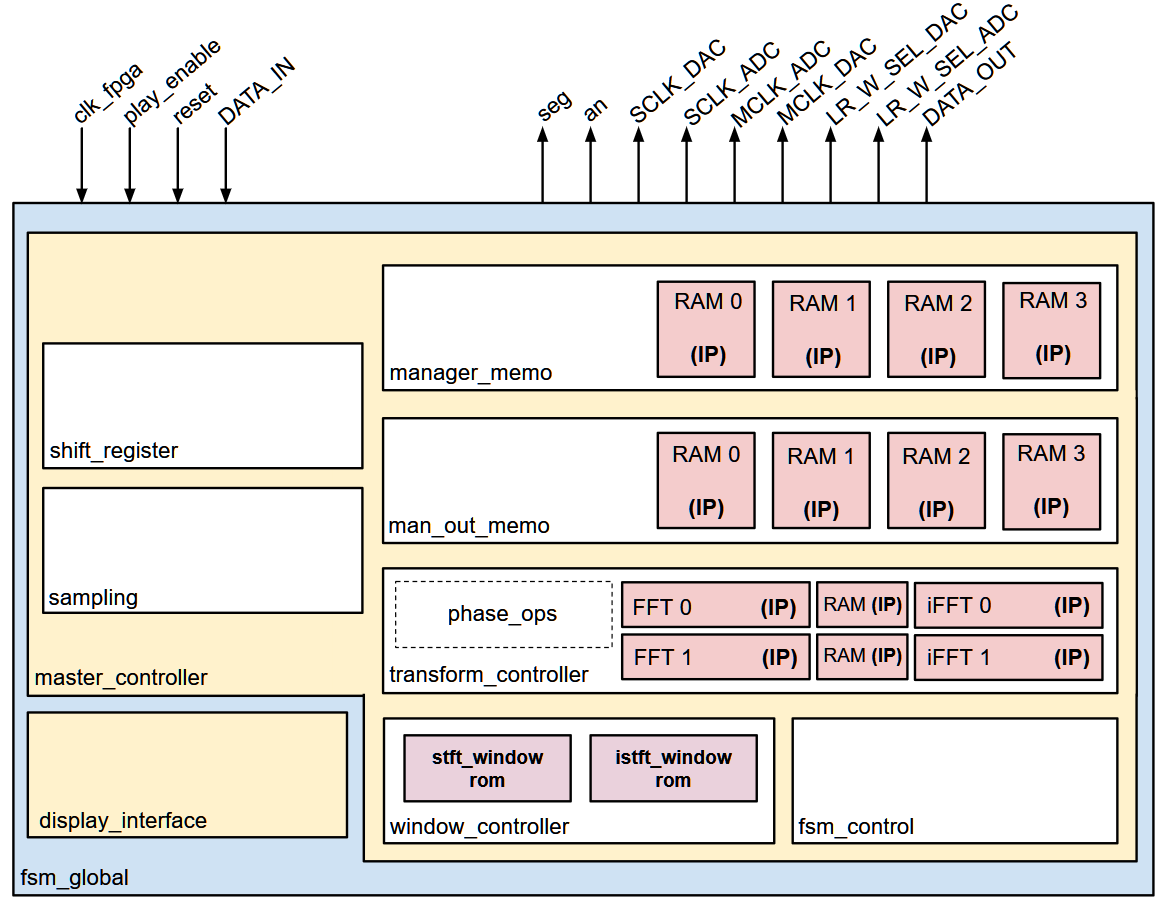
\includegraphics[width=15cm]{img/bloquesImp.png}
\caption{\label{fig:bimp}Estructura del código implementado}
\end{center}
\end{figure}

La figura \ref{fig:bimp} describe los ficheros VHDL empleados para implementar la operativa descrita previamente en la figura \ref{fig:dbloques} a excepción del módulo de operaciones sobre la fase, \emph{phase\_ops}, que se encuentra punteado. En ella se aprecian las señales de entrada y de salida globales, usando mayúsculas para las utilizadas por el Pmod i2-s2. Todos los ficheros utilizados se encuentran en su apéndice correspondiente al final del documento. Finalmente se detalla el funcionamiento de los displays utilizados.

\subsection{Displays}
El fichero \emph{display\_interface} será el que controle el manejo de los \emph{displays}. En este caso, únicamente va a leer la variable del estado global y modificar el mensaje de las pantallas en consecuencia entre \emph{play} y \emph{pause}. Existe gran documentación y ejemplos de como es el funcionamiento de estos \emph{displays} pero se ha utilizado la literatura proporcionada por Xillinx \cite{Nexys} para su implementación. Esta utiliza dos señales principales:
\begin{itemize}
\item \textbf{an:} Tiene 8 bits y controla qué display se va a emplear en cada instante. Por ello, debe ir conmutando entre todos ellos a una frecuencia lo suficientemente alta como para que resulte imperceptible al ojo. En este caso, se ha implementado un contador de 250000 que a una frecuencia de $100 MHz$ se corresponde con un periodo de refresco de $20 ms$.
\item \textbf{seg:} Es la señal que contiene la información sobre los segmentos que se van a iluminar, por lo que posee 7 bits, uno para cada segmento. Debe variar junto con la señal \emph{an} para que se muestre la información correcta en el display apropiado en cada momento.
\end{itemize}

Las asignaciones a estas señales siguen una lógica combinacional que solo dependen del estado global y de la cuenta que se realiza para actualizar el valor de \textbf{\emph{an}}. Cuando se alcanza el final de dicha cuenta, se actualiza el valor de \textbf{\emph{an}} de forma que se desplaza hacia la izquierda. El valor de \textbf{\emph{seg}} se almacena en 8 registros de forma que se utilice el correspondiente a cada valor de \textbf{\emph{an}}, tal y como muestra la figura \ref{fig:seg_an}.
\begin{figure}[!ht]
\begin{center}
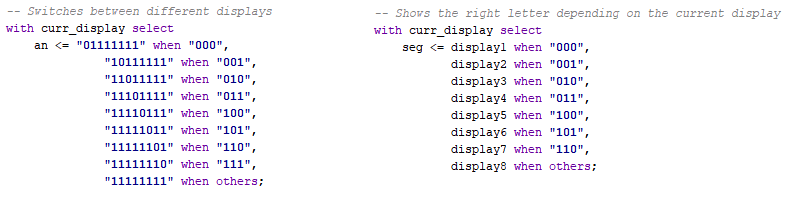
\includegraphics[width=16cm]{img/segan.png}
\caption{\label{fig:seg_an}Asignación de valores a las señales \textbf{\emph{an}} (derecha) y \textbf{\emph{seg}} (izquierda).}
\end{center}
\end{figure}

En esta figura también se puede ver su funcionamiento activo a nivel bajo. Finalmente, basta con asignar el valor adecuado a la señal de cada uno de los \emph{displays} que se va a introducir en \textbf{\emph{seg}}. Para ello se han creado una serie de constantes en el fichero de librería del proyecto, \emph{project\_trunk}, que contienen la codificación de cada uno de los caracteres que se van a emplear, para facilitar su programación.